\section{}



\subsection{}

Mithilfe der \texttt{interpolate}-Methode, die in SymPy bereits zur Verfügung steht, erhalten wir den folgenden Code zum Interpolieren mit $n$ auf $[-1,1]$ gleichmäßig verteilten Punkten:

\lstinputlisting[style=pythoncode, firstline = 1, lastline = 14]{chapter_09/exercise_09_47.py}

Wir testen unsere Funktion für die Werte $n = 5, 11, 17$ mit dem folgenden Code:

\lstinputlisting[style=pythoncode, firstline = 19, lastline = 21]{chapter_09/exercise_09_47.py}

Wir erhalten hierdurch die folgenden Graphen:

\begin{center}
  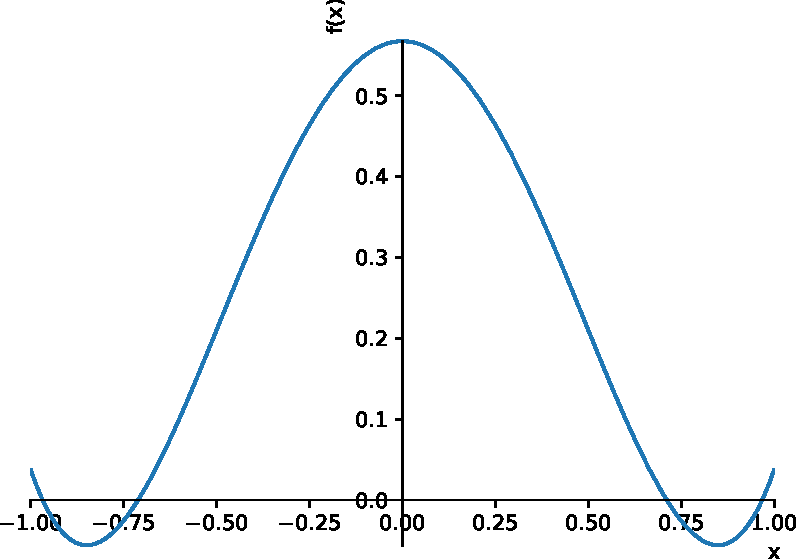
\includegraphics[width = 0.3\textwidth]{chapter_09/exercise_09_47_figure_1.pdf}
  \hspace{1em}
  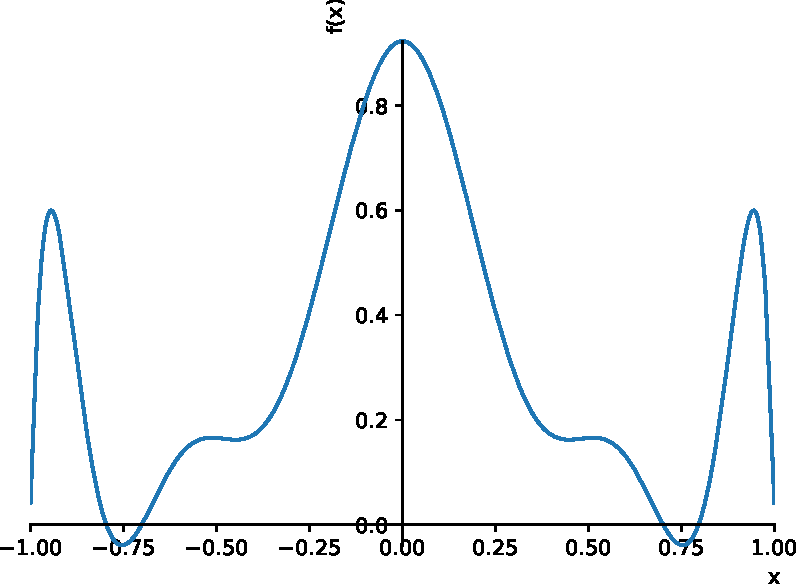
\includegraphics[width = 0.3\textwidth]{chapter_09/exercise_09_47_figure_2.pdf}
  \hspace{1em}
  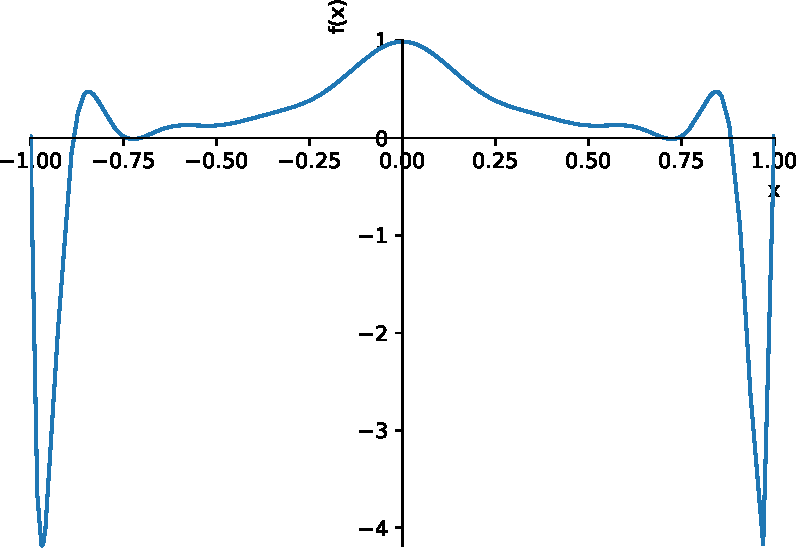
\includegraphics[width = 0.3\textwidth]{chapter_09/exercise_09_47_figure_3.pdf}
\end{center}

Es fällt auf, dass die Interpolationen zu den Intervallrändern hin zunehmend stark oszilliert.



\subsection{}

Mithilfe des folgenden Codes betrachten wir den Unterschied $f(x) - P_n(x)$:

\lstinputlisting[style=pythoncode, firstline = 26, lastline = 28]{chapter_09/exercise_09_47.py}

Unsere Vermutung scheint sich zu bestätigen:

\begin{center}
  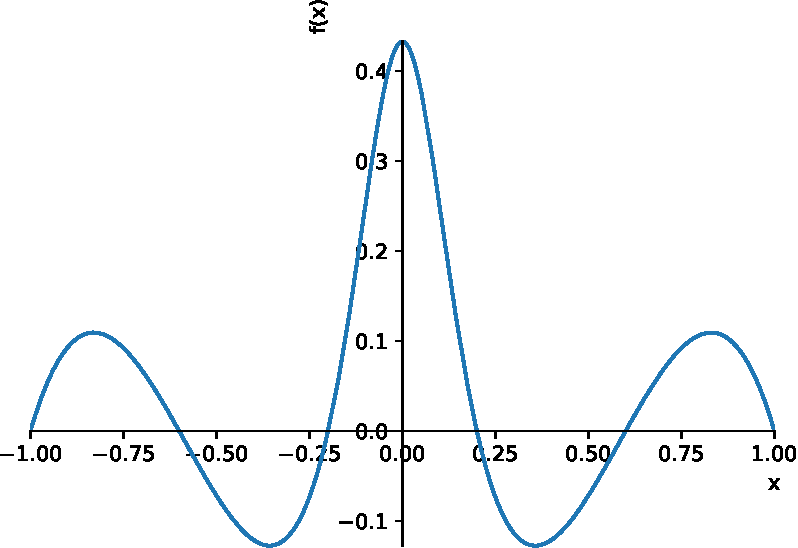
\includegraphics[width = 0.3\textwidth]{chapter_09/exercise_09_47_figure_4.pdf}
  \hspace{1em}
  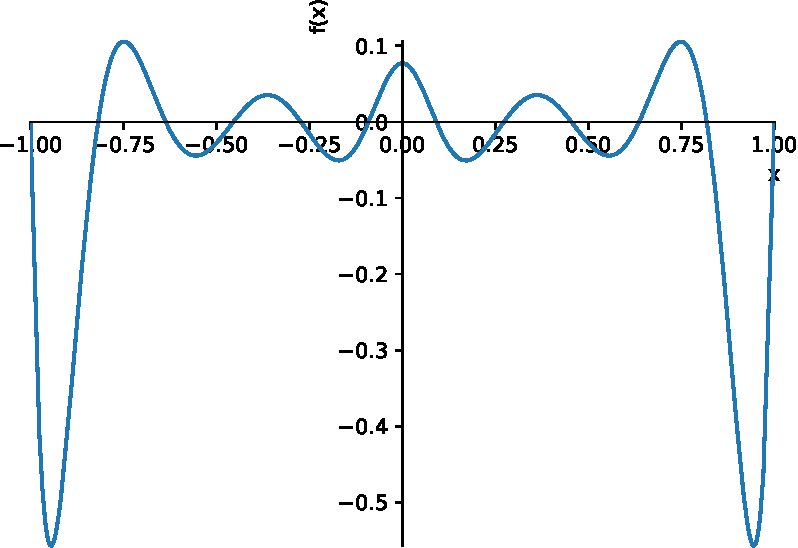
\includegraphics[width = 0.3\textwidth]{chapter_09/exercise_09_47_figure_5.pdf}
  \hspace{1em}
  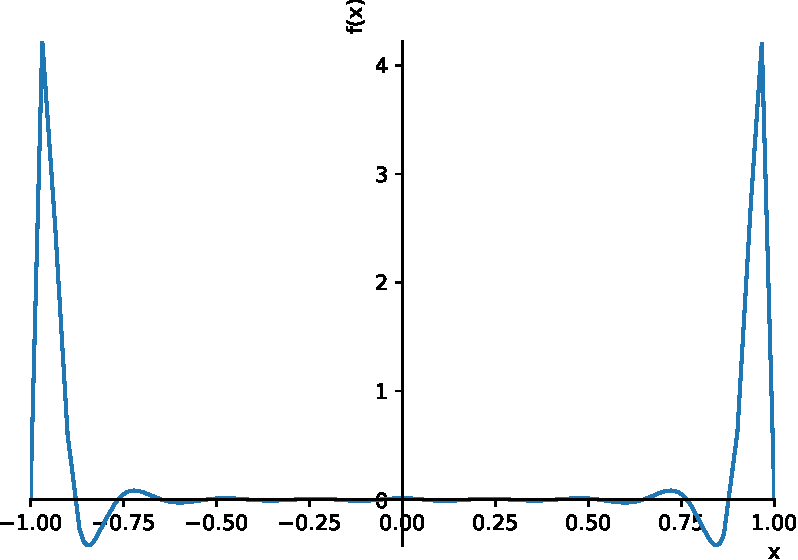
\includegraphics[width = 0.3\textwidth]{chapter_09/exercise_09_47_figure_6.pdf}
\end{center}
